% CVPR 2022 Paper Template
% based on the CVPR template provided by Ming-Ming Cheng (https://github.com/MCG-NKU/CVPR_Template)
% modified and extended by Stefan Roth (stefan.roth@NOSPAMtu-darmstadt.de)

\documentclass[10pt,twocolumn,letterpaper]{article}

%%%%%%%%% PAPER TYPE  - PLEASE UPDATE FOR FINAL VERSION
%\usepackage[review]{cvpr}      % To produce the REVIEW version
\usepackage{cvpr}              % To produce the CAMERA-READY version
%\usepackage[pagenumbers]{cvpr} % To force page numbers, e.g. for an arXiv version

% Include other packages here, before hyperref.
\usepackage{graphicx}
\usepackage{amsmath}
\usepackage{amssymb}
\usepackage{booktabs}
\usepackage{caption}
\usepackage{subcaption}

\usepackage[pagebackref,breaklinks,colorlinks]{hyperref}


% Support for easy cross-referencing
\usepackage[capitalize]{cleveref}
\crefname{section}{Sec.}{Secs.}
\Crefname{section}{Section}{Sections}
\Crefname{table}{Table}{Tables}
\crefname{table}{Tab.}{Tabs.}


%%%%%%%%% PAPER ID  - PLEASE UPDATE
\def\cvprPaperID{***} % *** Enter the CVPR Paper ID here
\def\confName{ x}
\def\confYear{2022}


\begin{document}
	
%%%%%%%%% TITLE - PLEASE UPDATE
\title{Visual Geo-Localization}

\author{Matteo Gambino\\
	s287572
	\and
	Michele Pierro\\
	s287846
	\and
	Fabio Grillo\\
	s287873
}
\maketitle

%%%%%%%%% ABSTRACT
\begin{abstract}
	In order to predict the location of a query image by retrieving annotated photographs with 
	similar descriptors needs an efficient and reliable generation of those descriptors. 
	In order to accomplish that objective, is fundamental that the network focuses on portion
	of the various images that contains useful information and at the same time ignore not 
	informative areas like the ones containing elements like cars or pedestrians. For that 
	reason attention layers are fundamental in the proposed network. In addition to that we 
	are comparing state of the art techniques for the visual geolocalization task like GeM \cite{GEM}, 
	NetVLAD \cite{NETVLAD} and CRN \cite{CRN}. The code used is publicly available 
	\href{https://github.com/matteo6198/project_visual_geolocalization}{here}
\end{abstract}

%%%%%%%%% BODY TEXT
\section{Introduction}

\section{Related works}

\section{Methods}
Like \cite{GEM}, \cite{NETVLAD}, \cite{CRN} we have casted the problem of place recognition as the task of image
retrieval. We have implemented 3 different networks all based on the ResNet-18 \cite{resnet} backbone
without the fully connected layers and the last convolution layer. On the top of this backbone we 
have inserted 4 different heads, inspired by the works of \cite{GEM}, \cite{NETVLAD}, \cite{CRN}, in order
to generate the image descriptors. 

\subsection{Base Head}
This is the simplest head we have used and it's necessary in order to have a baseline to compare the other
results. After the last convolution layer of ResNet-18 we have normalized the feature map and used average 
pooling in order to generate the descriptors. This simple head tries to extract from the query the spatial
information by comparing the average value of the features in a given area and represent the traditional way 
to extract those descriptors.

\subsection{GeM head}
Following the work of \cite{GEM}, we have used a Generalized Mean approach in order to extract better 
descriptors for the query image. The generalized mean we are using is defined as:
\begin{equation}
	f_k = ({\frac{1}{X_k}} \sum_{x \in X_k} x^{p_k} ) ^ {\frac{1}{p_k}}
\end{equation}
where $X_k $ represent one of the normalized features map and $p_k $ is the pooling parameter. This 
pooling parameter is expressing how much is localized the zone of the image the network is focusing on.
The $p_k $ parameter, although it can be learned and inserted into back propagation, it has been fixed
and a single value is used for each activation map as suggested by \cite{GEM}. We have
inserted a fully connected layer that takes as input the pooled features in order to whiten the image
descriptors since it has been shown by \cite{GEM} that this approach is providing better results than
using other strategies like PCA.

\subsection{NetVLAD head}\label{sec:NETVLAD}
Inspired by the work presented in \cite{NETVLAD}, we have implemented also a NetVLAD head that solves in an 
elegant way the problem of computing Vectors of Locally Aggregated Descriptors (VLAD), as described in \cite{VLAD},
in CNN. This network, in order to compute those VLAD descriptors, is using two different parts. 
The first is called soft-assignment branch that is replacing the hard assignment of a descriptor to a single cluster
with a soft assignment of the descriptor to every cluster. This is performed using a soft-max operation on top of the output of a $1x1$
convolution layer that produces the probabilities $s_k$ that a given descriptor $x_i$ belongs to a cluster $k$ by:
\begin{equation}
	s_k(x_i) = {{e^{W_k^T x_i+b_k}}\over{\sum_{k'} e^{W_{k'}^T x_i+b_{k'}}}}
\end{equation} 
The second part, denominated VLAD core, is effectively computing the 
VLAD representation of the image given an image descriptor $x$, the cluster centers $c$ and the computed soft assignments
$s$ following the equation:
\begin{equation}
	V(j,k) = \sum_{i=1}^N s_k(x_i) (x_i(j) - c_k(j))
\end{equation} 
where $x_i(j)$ and $c_k(j)$ represent respectively the j-th dimension of the i-th descriptor and the k-th cluster center.
The obtained descriptors are then intra-normalized (using a column-wise L-2 norm), flattened into a vector and then a
final L-2 norm operation is applied.
For this network is fundamental to initialize the cluster centers in order to obtain good performances. This initialization
is preformed in a preliminary step using a small subset of the training data available and consists in computing the features 
representations, using the pre-trained ResNet-18 backbone, and then extracting the descriptors by randomly selecting some of the 
obtained features. Then, in order to obtain the cluster's centroids, k-means is used over the computed descriptors and the 
weights in the convolution layer for soft-assignment are initialized, to reproduce the results that would have been obtained
with VLAD described in \cite{VLAD}, using:
\begin{equation}
   W = \alpha ({\frac{c}{{||c||}_2}} \cdot d )
\end{equation}
where $c$ and $d$ are respectively the computed clusters centers and descriptors, $\alpha$ is instead selected to be large
in order to better mimic the traditional VLAD.

\subsection{CRN head}
Seen the results provided from the previous implemented heads and the success of the attention layers to make 
a network focus on relevant only parts of an image, we have decided to add an attention layer at the NetVLAD
head following the approach proposed by \cite{CRN}. This is perfectly integrated in the NetVLAD architecture and
it has the duty to produce a map that rescales the weights produced by the soft assignment step of the NetVLAD layer.
This layer is composed by an initial average pooling sub-layer
that has the duty to reduce the dimensionality of the feature maps produced by the backbone. 
Differently from what specified in \cite{CRN}, it is not reducing the features maps to a fixed 
size but it is simply reducing by a half the dimensions of the features. In order to capture features at different
spatial resolutions, $3$ convolution filters (with kernel sizes respectively of $3$, $5$, $7$) are applied to the pooled features.
The  output of those filter is concatenated and an additional $1x1$ convolution filter is used in order to accumulate the 
features produced. The resulting mask is then upsampled, in order to restore the original features map dimensionality,
by using a bilinear interpolator.This results into a mask that is used as to re-weight the features produced by the soft assignment specified
into the NetVLAD description as showed in figure \ref{fig:CRN:ark} into the context modulation layer. This layer is 
performing the product of the mask and the soft-assignment scores. The output of the context modulation layer is then used 
in the standard NetVLAD core instead of the soft-assignment scores. Also this head requires the initialization of centroids as the 
NetVLAD head and the initialization adopted is the same described in the section \ref{sec:NETVLAD}.

\begin{figure}
	\centering
	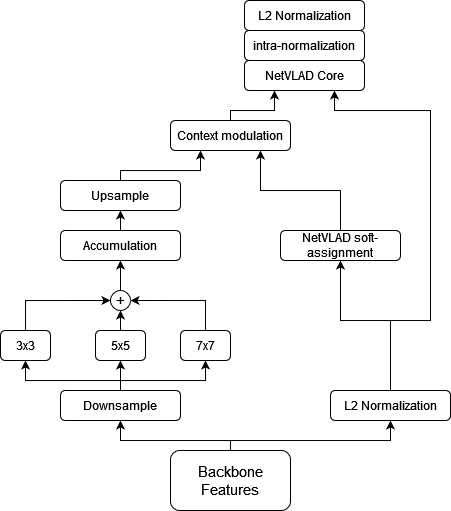
\includegraphics[width=0.3\textwidth]{img/CRN.png}
	\caption{The architecture of the CRN head.}
	\label{fig:CRN:ark}
\end{figure}

\subsection{CRN2 head}
In order to reduce the number of parameters to be learned by the CRN head, we have implemented a second version of this head,
called CRN2, that exploits the ideas of concatenating multiple $3x3$ filters in order to obtain the same receptive field of a
bigger filter but using less parameters as suggested in \cite{VGG}. In particular we have replaced the $5x5$ and the $7x7$ filters showed in figure \ref{fig:CRN:ark}
with respectively 2 and 3 stacked $3x3$ filters as showed in figure \ref{fig:CRN2:ark}. In addition to that, we have used dilated convolution
in order to remove the pooling and upsampling layers by generating the mask directly at the desired resolution inspired by the work 
proposed in \cite{atrous}. This, although requires 
more computation, will produce more accurate masks that may help the network to better focus on the relevant parts of the images.
Also this head requires the initialization of centroids as the CRN and the NetVLAD heads
and the initialization adopted is the same described in the section \ref{sec:NETVLAD}.

\begin{figure}
	\centering
	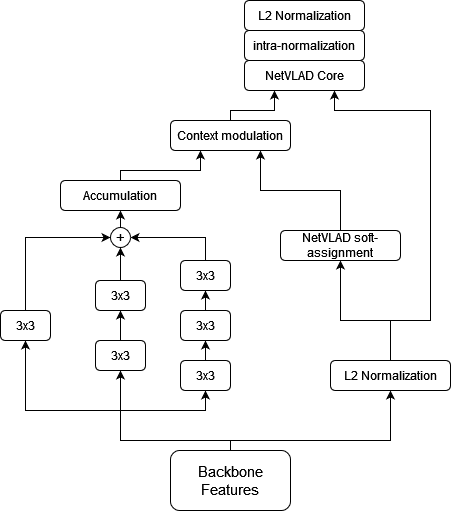
\includegraphics[width=0.3\textwidth]{img/CRN2.png}
	\caption{The architecture of the CRN2 head.}
	\label{fig:CRN2:ark}
\end{figure}

\section{Experiments}
In this section we evaluate the results obtained by the implemented heads and the selection of best hyper-parameters will be discussed.

\begin{figure}
	\centering
	\begin{subfigure}[b]{0.23\textwidth}
		\centering
		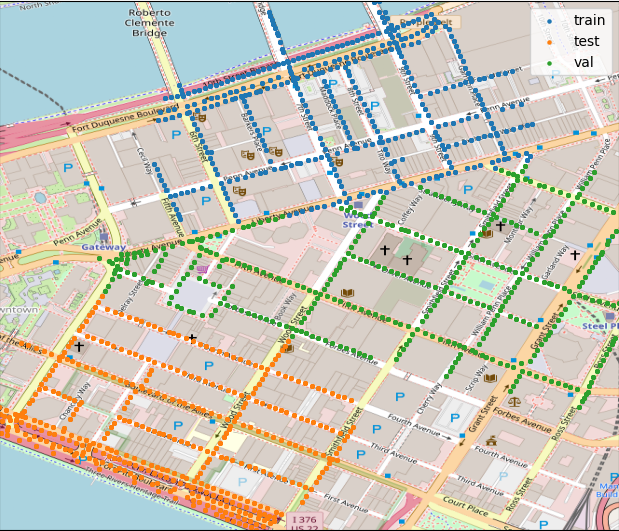
\includegraphics[width=\textwidth]{img/pitts_out.png}
		\caption{Pitts30k}
		\label{fig:datasets:pitts30k}
	\end{subfigure}
	\hfill
	\begin{subfigure}[b]{0.23\textwidth}
		\centering
		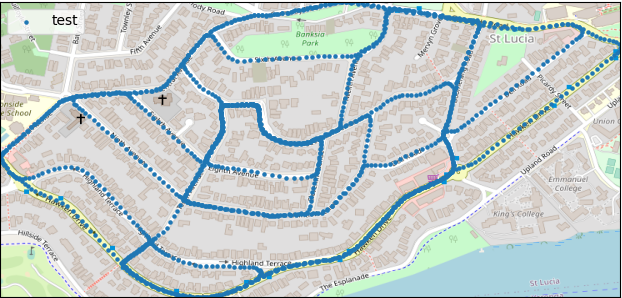
\includegraphics[width=\textwidth]{img/st_lucia_out.png}
		\begin{minipage}{1cm}
			\vfill
		\end{minipage}
		\vspace{0.2cm}
		\caption{St. Lucia}
		\label{fig:datasets:st_lucia}
	\end{subfigure}
	\caption{The location of the images contained in both the pitts30k \ref{fig:datasets:pitts30k} dataset and the St. Lucia \ref{fig:datasets:st_lucia} dataset.}
	\label{fig:datasets}
\end{figure}

\paragraph{Datasets}
The experiments have been run on the pitts30k dataset \cite{NETVLAD} that is containing 3 different predefined splits, respectively for 
training, validation and testing, composed by $10k$ images each. Those are images taken in the city of Pittsburgh from the Google street
view images. In addition, also the St. Lucia dataset \cite{st_lucia} has been used only for testing the models trained on the pitts30k dataset.
The location of the images contained in both datasets can be seen in figure \ref{fig:datasets}.

\paragraph{Mining procedure}\label{par:mining}
In order to train our models we need to generate triplets in the form $\{I_q, I^+, I^-\}$: for each query image $I_q$ we are looking for
positive examples $I^+$ and negative ones ($I^-$). In order to do so, for each query image we retrieve the images into the database that are
in a range specified by the positive distance threshold. We use 2 possibly different values for this threshold at train and test time.
Among all images in this range, we select as best positive the one that has descriptors more similar to the query image and we use this image
as $I^+$. All the images not in the positive distance threshold range are considered as negative samples. We select by default the 10 
images, from the negative set, that have the as similar as possible descriptors as the query image. We call those images hard negatives and
we are using those instead of randomly picking from the negative set in order to make the task for the network more challenging resulting in 
a more robust model. Since we have to generate the descriptors that vary over the training procedure, we are periodically recalculating the 
triplets within the epochs.
\paragraph{Loss function}
We have set the problem of visual geo-localization in approximating the location of a query image by retrieving the nearest 
database images in the descriptors space. For that reason, the objective of our training procedure is to make images geographically
close have a similar representation in descriptor space and instead make as far as possible the representation of geographically far images.
This is possible by exploiting contrastive learning and the loss function that we are using is defined by
\begin{equation}
   L(q, p, n) = \sum_i max( {|| q - p ||}_2 - {|| q - n_i||}_2 + m, 0)
\end{equation}
where $p$, $q$ and $n_i$ represent the descriptors extracted by the query image, the positive image and the negative ones (by default we extract
$10$ negatives examples for each query image as described in \nameref{par:mining}).
The parameter $m$ is instead specifying a margin between the positive and negative descriptor representation of the images.
In fact, if a negative sample has a distance in the descriptors space higher than the margin $m$ the resulting loss will be $0$ and, instead,
if the distance between the positive and negative descriptors is lower than the margin the loss will be proportional to the margin violation.

\paragraph{Metric adopted}
Those results have been obtained by evaluating the models by using a standard evaluation procedure for place recognition.
A given query image is said to be correctly localized if at least one of the $N$ retrieved images is placed at a distance lower
or equal to $TTD$ from the ground truth position. This distance is set, if not differently specified, to $25$ meters. After
that we are calculating the percentage of correctly classified images for different values of $N$ (indicated with $R@N$).  

\subsection{Comparison among the proposed heads}
The results of comparison between the various proposed heads are reported in table \ref{tab:base_results}. Those results have 
been obtained on the pitts30k test set. As it's possible to notice the head that is giving best results is the CRN and that 
shows that adding attention is essential for improving the quality of generated descriptors. It's important to notice also how 
the results are influenced by the number of produced descriptors. In fact both the NetVLAD and the CRN head are generating much 
more descriptors with respect to the GeM and the base heads and this seems correlated to higher recalls. Since the CRN and the NetVLAD
heads are outperforming the other ones, we will focus more on those 2 during the rest of this section.

\begin{table}
	\centering
	\begin{tabular}{|l|c|c|c|c|c|}
		\hline
		& Descs.&        $R@1$   &        $R@5$   &        $R@10$  &        $R@20$   \\ \hline
		Base     & 256   &         60.1   &         80.6   &          87.4   &          91.7   \\
		GeM      & 256   &         71.6   &         87.0   &          91.0   &          94.0   \\
		NetVLAD  & 16384 &         79.1   &         89.3   &          92.3   &          94.4   \\ \hline
		CRN*     & 16384 &         81.7   & \textbf{90.7}  &  \textbf{93.4}  &  \textbf{95.3}  \\
		CRN2     & 16384 &\textbf{81.8}   & \textbf{90.7}  &          93.2   &          95.2   \\ \hline
	\end{tabular}
	\caption{Results on the pitts30k test set obtained with the various heads compared with the base head. The number of generated descriptors 
		is also shown in the column Descs.}
	\label{tab:base_results}
\end{table}

\subsection{CRN and CRN2 models}
As it's possible to notice from table \ref{tab:base_results}, the performances of the CRN and CRN2 networks are very close one to each other as expected
from the definition of the two networks. It's important to notice that the CRN2 network is using less parameters with respect to the CRN network. In fact,
the CRN2 network is using only 245K parameters compared to the 529k parameters used by the CRN network for the generation of the mask.
As shown in the table \ref{tab:time}, the time required to extract descriptors for a single image is higher for the CRN2 network with an increase of 32.5\% 
of the required execution time. This is due to the removal of the downsampling layer present in the original CRN implementation that implies the analysis of the image 
at full resolution and this 
has to be taken in consideration during the deploy phase where the descriptors for the query images have to be computed online. We have also noticed that an increase
of the time required to produce descriptors is correlated to better recalls values and also this has to be taken in consideration while deploying an 
application using those networks.

\begin{table}
   \centering
   \begin{tabular}{|l|c|}
      \hline
      Network     &  time (s)\\\hline
      Base       &  0.0158\\
      GeM        &  0.0158\\
      NetVLAD     &  0.0206\\
      CRN         &  0.0215\\
      CRN2        &  0.0285\\\hline
   \end{tabular}
   \caption{The running time for computing the descriptors of a single image for the various networks computed on a GPU NVIDIA Tesla K80.}
   \label{tab:time}
\end{table}

	
\section{Ablation study}
In this section we discuss the effect of changing one by one some paramethers of the NetVLAD network, we expecially focused on trying different learning rates, modifying the distance at which positives are taken.\\ We also changed the input images of the dataset by implementing some data augmentation tecniques and by changing the resolution of the images.\\
As optimizer algorithm we decided to use the Stochastic gradient descent (SGD), the results of the application of this iterative method are clear in terms of recall, in the table is possible seeing an increment of it in both the datasets.\\
pitts30k
\begin{table}[!h]
	\centering
	\begin{tabular}{|l|c|c|c|c|}
		\hline
		.&        $R@1$   &        $R@5$   &        $R@10$  &        $R@20$   \\ \hline
		NetVLAD  Pitts30k     &         60.1   &         79.7   &          86.4   &          91.2   \\
		NetVLAD St. Lucia        &         24.2   &         43.3   &          53.7   &          65.3   \\ \hline
		NetVLAD (SGD) Pitts30k  &         79.5   &         90.4   &          93.0   &          95.0   \\ 
		NetVLAD (SGD) St. Lucia      &         42.1   & 56.8  &  63.7  &  71.4  \\
		 \hline
	\end{tabular}
	\caption{Results on the pitts30k and St. Lucia test sets obtained with the NetVLAD head compared with the NetVLAD+SDG head.}
	\label{tab:base_results}
\end{table}

\subsection{Comparison between different learning rates}
As first ablation study we tried different learning rates, from the table we can see that the best results in calculating the percentage of correctly classified images are obtained with a learning rate of 1 , with this learning rate the network is superior to the other configuration of learning rate in each case. We also noticed that by decreasing the learning rate we increment the number of epochs needed to end the training.
\begin{table}[!h]
	\centering
	\begin{tabular}{|l|c|c|c|c|}
		\hline
		&          $R@1$  &        $R@5$  &        $R@10$ &        $R@20$   \\ \hline     
		lr = 1e-3 &         78.6    &    89.4       &    92.5       &         94.7       \\
		lr = 1e-4 &         60.0    &         79.7  & 86.4 & 91.2  \\    
		lr = 1e-5 & \textbf{82.3}   & \textbf{92.7} &         \textbf{95.0}  & \textbf{97.0}          \\
		\hline
	\end{tabular}
	\caption{Results obtained with the NetVLAD head on the pitts30k test set with different learning rates}
	\label{tab:NETVLAD:lr}
\end{table}
\subsection{Comparison between different positive distance treshold}
Initially the distance at which positive are taken was set at 25 meters, we tried to change the parameter ${val\_positives\_dist\_threshold}$ with different values. The graph contained in figure 6 shows that, during training, the positive distance threshold set at 5 meter outperforms all the other thresholds in every recall in both the Pitts30k and St Lucia datasets.\\
\begin{figure}[!h]
	\centering
	\begin{subfigure}[b]{0.23\textwidth}
		\centering
		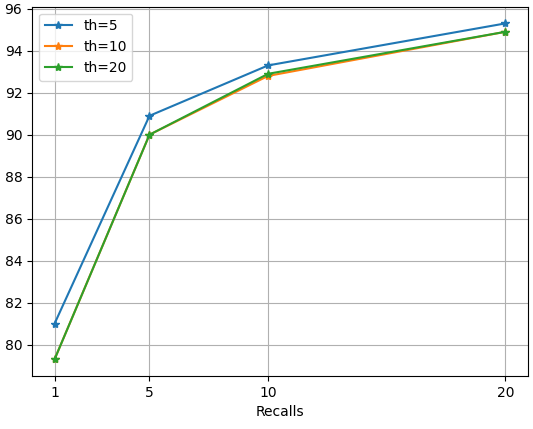
\includegraphics[width=\textwidth]{img/train_th/test_pitts30k_recalls_graph.png}
		\caption{Pitts30k}
		\label{fig:recalls:train_th:pitts30k}
	\end{subfigure}
	\hfill
	\begin{subfigure}[b]{0.23\textwidth}
		\centering
		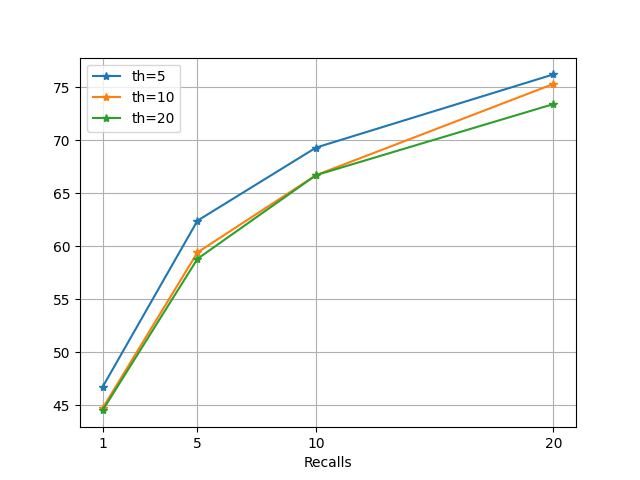
\includegraphics[width=\textwidth]{img/train_th/test_st_lucia_recalls_graph.png}
		\caption{St. Lucia}
		\label{fig:recalls:train_th:st_lucia}
	\end{subfigure}
	\caption{Graph showing the recalls obtained with different train positive distance threshold on both the pitts30k \ref{fig:recalls:train_th:pitts30k} dataset and the St. Lucia \ref{fig:recalls:train_th:st_lucia} dataset.}
	\label{fig:recalls:train_th}
\end{figure}
We also tried different test positive distance threshold and in this case there is a big difference between the different distances, greater distances perfom in a better way than smaller ones.\\
By setting a larger positive distance we have worse performances because it leads to an increase in the false positives.
\begin{figure}[!h]
	\centering
	\begin{subfigure}[b]{0.23\textwidth}
		\centering
		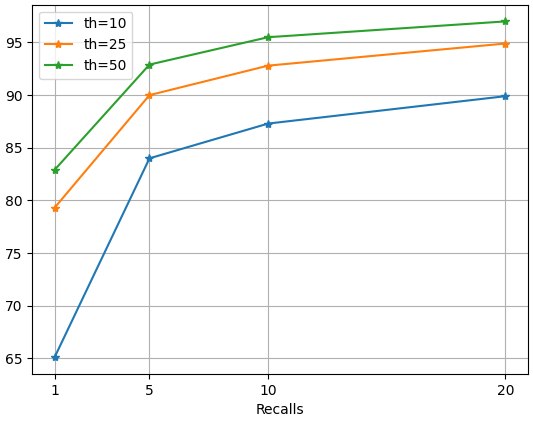
\includegraphics[width=\textwidth]{img/test_th/test_pitts30k_recalls_graph.png}
		\caption{Pitts30k}
		\label{fig:recalls:test_th:pitts30k}
	\end{subfigure}
	\hfill
	\begin{subfigure}[b]{0.23\textwidth}
		\centering
		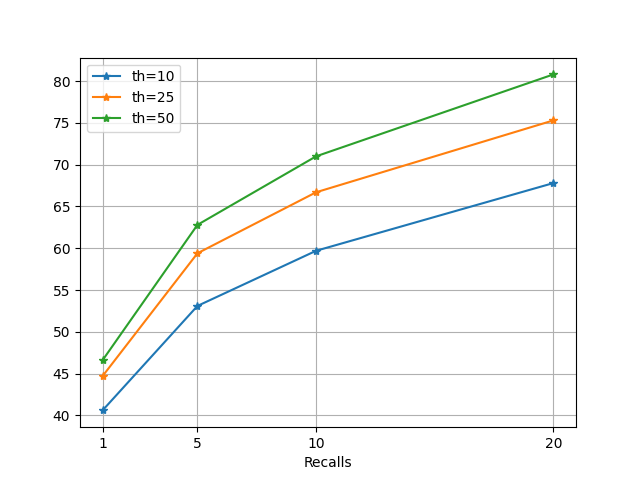
\includegraphics[width=\textwidth]{img/test_th/test_st_lucia_recalls_graph.png}
		\caption{St. Lucia}
		\label{fig:recalls:test_th:st_lucia}
	\end{subfigure}
	\caption{Graph showing the recalls obtained with different test positive distance threshold on both the pitts30k \ref{fig:recalls:test_th:pitts30k} dataset and the St. Lucia \ref{fig:recalls:test_th:st_lucia} dataset.}
	\label{fig:recalls:test_th}
\end{figure}
In the Pitts30k dataset we can see that the recall on one image is 65.1 with the positive threshold distance set at 10 meters while the recall with the distance set at 50 meters is 82.9, there is a margin of 17.8\%\\
The same trend is mantained in all the different recalls on both the Pitts30k and St. Lucia datasets, but while in the Pitts30k the margin between the distance treshold set at 10 meters and the one set at 50 meters stabilizes, in the St Lucia Datasets keeps incrementing, initially it's 6\% at R1 and becomes 13\% at R20.

\subsection{Comparison between different data augmentation tecniques}
In order to see how the results change we tried some data augmentation techniques, we decided to use 3 of them: Color Jitter, Horizontal Flip + Rotate and Random Erasing. With Color Jitter we randomized the contrast and brightness of the image, with Horizontal Flip we flipped the image over the vertical axis and with the last trasformation we erase with random values the pixel contained inside a rectangle region.\\
\begin{figure}[!h]
	\centering
	\begin{subfigure}[b]{0.23\textwidth}
		\centering
		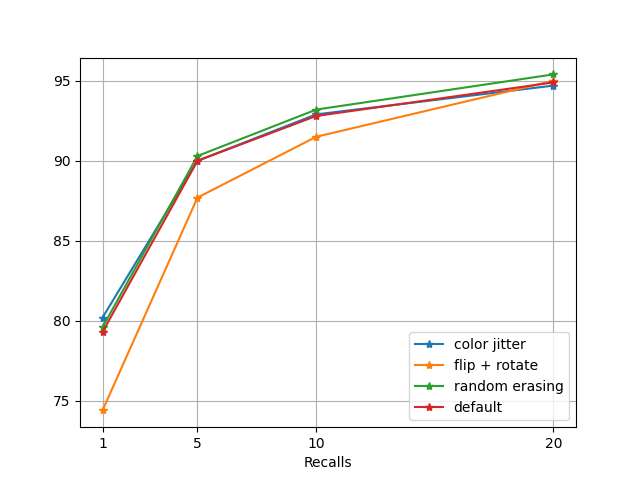
\includegraphics[width=\textwidth]{img/augment/test_pitts30k_recalls_graph.png}
		\caption{Pitts30k}
		\label{fig:recalls:augment:pitts30k}
	\end{subfigure}
	\hfill
	\begin{subfigure}[b]{0.23\textwidth}
		\centering
		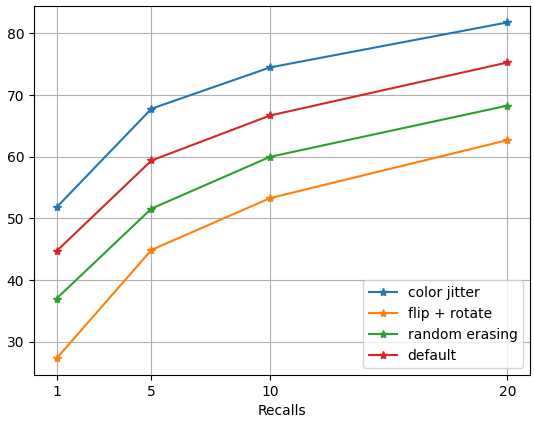
\includegraphics[width=\textwidth]{img/augment/test_st_lucia_recalls_graph.png}
		\caption{St. Lucia}
		\label{fig:recalls:augment:st_lucia}
	\end{subfigure}
	\caption{Graph showing the recalls obtained with different augmentation techniques on both the pitts30k \ref{fig:recalls:augment:pitts30k} dataset and the St. Lucia \ref{fig:recalls:augment:st_lucia} dataset.}
	\label{fig:recalls:augment}
\end{figure}
For the Pitts30k dataset we can see in figure \textcolor{red}{5a} that all the data augmentation techniques have a similar performance compared to the default configuration of the dataset; Only the flip and rotate technique gets sightly worse results in the first recalls.\\
For the St. Lucia dataset we can see in figure \textcolor{red}{5b} that all the data augmentation techniques have very different performance, in this case only the Color Jitter transformation gets better results than the default configurations, while  Random Erasing and Flip + Rotate get sightly worse results in all the recalls.\\
The Color Jitter tecnique is the only tecnique that gets better results because it's the only one that does not change the structure of the images.

\subsection{Comparison between different images sizes}
The last ablation study has been the variation of the images sizes by scaling their dimensions by a scaling factor. We decided to try 4 scaling factors (including the standard one 1.00), the value selected are: 0.50, 0.75, 1.00, and 1.25.\\
The results of the scaling factor are shown in figure \textcolor{red}{7}, for both the Pitts30k and St. Lucia dataset it's clear that a reduction of the image size leads to an increment in the recall's value; This increment is way more visible in the St. Lucia dataset (figure \textcolor{red}{7b}).
	\begin{figure}[!h]
	\centering
	\begin{subfigure}[b]{0.23\textwidth}
		\centering
		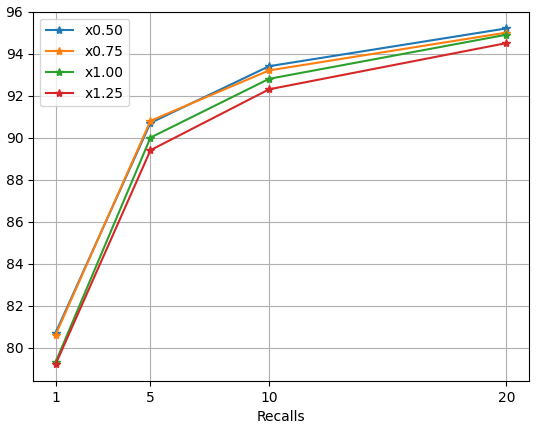
\includegraphics[width=\textwidth]{img/resize/test_pitts30k_recalls_graph.png}
		\caption{Pitts30k}
		\label{fig:recalls:resize:pitts30k}
	\end{subfigure}
	\hfill
	\begin{subfigure}[b]{0.23\textwidth}
		\centering
		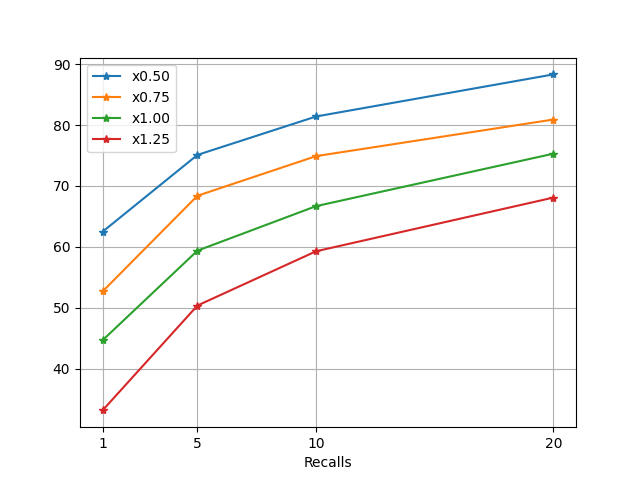
\includegraphics[width=\textwidth]{img/resize/test_st_lucia_recalls_graph.png}
		\caption{St. Lucia}
		\label{fig:recalls:resize:st_lucia}
	\end{subfigure}
	\caption{Graph showing the recalls obtained with different input image size on both the pitts30k \ref{fig:recalls:resize:pitts30k} dataset and the St. Lucia \ref{fig:recalls:resize:st_lucia} dataset.}
	\label{fig:recalls:resize}
\end{figure}

\section{Conclusions}

%%%%%%%%% REFERENCES
{\small
	\bibliographystyle{ieee_fullname}
	\bibliography{egbib}
}
	
\end{document}